\documentclass[]{article}
\usepackage{lmodern}
\usepackage{amssymb,amsmath}
\usepackage{ifxetex,ifluatex}
\usepackage{fixltx2e} % provides \textsubscript
\ifnum 0\ifxetex 1\fi\ifluatex 1\fi=0 % if pdftex
  \usepackage[T1]{fontenc}
  \usepackage[utf8]{inputenc}
\else % if luatex or xelatex
  \ifxetex
    \usepackage{mathspec}
  \else
    \usepackage{fontspec}
  \fi
  \defaultfontfeatures{Ligatures=TeX,Scale=MatchLowercase}
\fi
% use upquote if available, for straight quotes in verbatim environments
\IfFileExists{upquote.sty}{\usepackage{upquote}}{}
% use microtype if available
\IfFileExists{microtype.sty}{%
\usepackage{microtype}
\UseMicrotypeSet[protrusion]{basicmath} % disable protrusion for tt fonts
}{}
\usepackage[margin=1in]{geometry}
\usepackage{hyperref}
\hypersetup{unicode=true,
            pdftitle={Extracción Actividades Emociones},
            pdfauthor={Ronald},
            pdfborder={0 0 0},
            breaklinks=true}
\urlstyle{same}  % don't use monospace font for urls
\usepackage{color}
\usepackage{fancyvrb}
\newcommand{\VerbBar}{|}
\newcommand{\VERB}{\Verb[commandchars=\\\{\}]}
\DefineVerbatimEnvironment{Highlighting}{Verbatim}{commandchars=\\\{\}}
% Add ',fontsize=\small' for more characters per line
\usepackage{framed}
\definecolor{shadecolor}{RGB}{248,248,248}
\newenvironment{Shaded}{\begin{snugshade}}{\end{snugshade}}
\newcommand{\AlertTok}[1]{\textcolor[rgb]{0.94,0.16,0.16}{#1}}
\newcommand{\AnnotationTok}[1]{\textcolor[rgb]{0.56,0.35,0.01}{\textbf{\textit{#1}}}}
\newcommand{\AttributeTok}[1]{\textcolor[rgb]{0.77,0.63,0.00}{#1}}
\newcommand{\BaseNTok}[1]{\textcolor[rgb]{0.00,0.00,0.81}{#1}}
\newcommand{\BuiltInTok}[1]{#1}
\newcommand{\CharTok}[1]{\textcolor[rgb]{0.31,0.60,0.02}{#1}}
\newcommand{\CommentTok}[1]{\textcolor[rgb]{0.56,0.35,0.01}{\textit{#1}}}
\newcommand{\CommentVarTok}[1]{\textcolor[rgb]{0.56,0.35,0.01}{\textbf{\textit{#1}}}}
\newcommand{\ConstantTok}[1]{\textcolor[rgb]{0.00,0.00,0.00}{#1}}
\newcommand{\ControlFlowTok}[1]{\textcolor[rgb]{0.13,0.29,0.53}{\textbf{#1}}}
\newcommand{\DataTypeTok}[1]{\textcolor[rgb]{0.13,0.29,0.53}{#1}}
\newcommand{\DecValTok}[1]{\textcolor[rgb]{0.00,0.00,0.81}{#1}}
\newcommand{\DocumentationTok}[1]{\textcolor[rgb]{0.56,0.35,0.01}{\textbf{\textit{#1}}}}
\newcommand{\ErrorTok}[1]{\textcolor[rgb]{0.64,0.00,0.00}{\textbf{#1}}}
\newcommand{\ExtensionTok}[1]{#1}
\newcommand{\FloatTok}[1]{\textcolor[rgb]{0.00,0.00,0.81}{#1}}
\newcommand{\FunctionTok}[1]{\textcolor[rgb]{0.00,0.00,0.00}{#1}}
\newcommand{\ImportTok}[1]{#1}
\newcommand{\InformationTok}[1]{\textcolor[rgb]{0.56,0.35,0.01}{\textbf{\textit{#1}}}}
\newcommand{\KeywordTok}[1]{\textcolor[rgb]{0.13,0.29,0.53}{\textbf{#1}}}
\newcommand{\NormalTok}[1]{#1}
\newcommand{\OperatorTok}[1]{\textcolor[rgb]{0.81,0.36,0.00}{\textbf{#1}}}
\newcommand{\OtherTok}[1]{\textcolor[rgb]{0.56,0.35,0.01}{#1}}
\newcommand{\PreprocessorTok}[1]{\textcolor[rgb]{0.56,0.35,0.01}{\textit{#1}}}
\newcommand{\RegionMarkerTok}[1]{#1}
\newcommand{\SpecialCharTok}[1]{\textcolor[rgb]{0.00,0.00,0.00}{#1}}
\newcommand{\SpecialStringTok}[1]{\textcolor[rgb]{0.31,0.60,0.02}{#1}}
\newcommand{\StringTok}[1]{\textcolor[rgb]{0.31,0.60,0.02}{#1}}
\newcommand{\VariableTok}[1]{\textcolor[rgb]{0.00,0.00,0.00}{#1}}
\newcommand{\VerbatimStringTok}[1]{\textcolor[rgb]{0.31,0.60,0.02}{#1}}
\newcommand{\WarningTok}[1]{\textcolor[rgb]{0.56,0.35,0.01}{\textbf{\textit{#1}}}}
\usepackage{longtable,booktabs}
\usepackage{graphicx,grffile}
\makeatletter
\def\maxwidth{\ifdim\Gin@nat@width>\linewidth\linewidth\else\Gin@nat@width\fi}
\def\maxheight{\ifdim\Gin@nat@height>\textheight\textheight\else\Gin@nat@height\fi}
\makeatother
% Scale images if necessary, so that they will not overflow the page
% margins by default, and it is still possible to overwrite the defaults
% using explicit options in \includegraphics[width, height, ...]{}
\setkeys{Gin}{width=\maxwidth,height=\maxheight,keepaspectratio}
\IfFileExists{parskip.sty}{%
\usepackage{parskip}
}{% else
\setlength{\parindent}{0pt}
\setlength{\parskip}{6pt plus 2pt minus 1pt}
}
\setlength{\emergencystretch}{3em}  % prevent overfull lines
\providecommand{\tightlist}{%
  \setlength{\itemsep}{0pt}\setlength{\parskip}{0pt}}
\setcounter{secnumdepth}{0}
% Redefines (sub)paragraphs to behave more like sections
\ifx\paragraph\undefined\else
\let\oldparagraph\paragraph
\renewcommand{\paragraph}[1]{\oldparagraph{#1}\mbox{}}
\fi
\ifx\subparagraph\undefined\else
\let\oldsubparagraph\subparagraph
\renewcommand{\subparagraph}[1]{\oldsubparagraph{#1}\mbox{}}
\fi

%%% Use protect on footnotes to avoid problems with footnotes in titles
\let\rmarkdownfootnote\footnote%
\def\footnote{\protect\rmarkdownfootnote}

%%% Change title format to be more compact
\usepackage{titling}

% Create subtitle command for use in maketitle
\providecommand{\subtitle}[1]{
  \posttitle{
    \begin{center}\large#1\end{center}
    }
}

\setlength{\droptitle}{-2em}

  \title{Extracción Actividades Emociones}
    \pretitle{\vspace{\droptitle}\centering\huge}
  \posttitle{\par}
    \author{Ronald}
    \preauthor{\centering\large\emph}
  \postauthor{\par}
    \date{}
    \predate{}\postdate{}
  

\begin{document}
\maketitle

\hypertarget{implicit-activities-and-emotions-in-prif-em}{%
\section{Implicit Activities and emotions in
PRIF-EM}\label{implicit-activities-and-emotions-in-prif-em}}

From the review of the works related to the measurement of physical and
psychological aspects in work and academic settings, a potential
opportunity is found, for the use of artificial intelligence as a
support component in the psycho-social assessment. The questionnaires
currently used for quantitative and qualitative assessment implicitly
contain activities, emotions, moods, and situations that the person
providing the test answers may experience. In this project, we will
limit ourselves to extracting the functional activities that are to
support the physical, social, and psychological well-being of a person
and allows that person to function in society {[}{]}. Additionally, they
will extract the Instrumental Activity of Daily Living (IADL), which is
defined as those activities that allow an individual to live
independently in a community. according{[}{]}. On the other hand, the
emotions within the items of the questionnaires will be extracted,
taking as reference the study of emotions by Paul Ekman {[}{]}.

\hypertarget{methodology-of-extraction}{%
\subsection{Methodology of extraction}\label{methodology-of-extraction}}

Como primer paso de la metodología de extracción se efectua un análisis
detallado de los mecanismo empleados en las publicaciones. Entre las
diferentes motivaciones para el uso de los mecanismos se encuentra la
validación en un segmento de problación especifico{[}{]}, el soporte
metodológico y de cuantificación para la validación experimental{[}{]}
soportada{[}{]} o la adaptación de todos o algunos de sus items en un
contexto definido{[}{]}. La motivación en este caso, será la de
identificar los cuestionarios mencionados en artículos que establecen su
enfoque en aspectos relacionados con los riesgos psicosociales en los
contextos laboral y académico. Posterior a esto, se extraen los dominios
de aplicación que agrupan los diferentes items o preguntas que son
efectuadas a las personas evaluadas. Cada item es analizado, con el fin
identificar las actividades, emociones y la frecuencia en la que se
presentan. Para orientar la extracción de dichas actividades y emociones
se toma como referencia el trabjo de Melzer{[}@MELZER2019{]} en el que
se aborda el reconocimiento de emociones a partir de los movimientos
corporales. Esta aproximación no sólo representa una referencia
metodológica, sino que encaja con el alcance del trabajo para la
identificación y caracterización de escenarios en los que se involucren
las acciones realizadas por personas y que puedan ser capturadas
mediante cámaras de video.

Dentro de las referencias seleccionadas se establece una separación en
los dos contextos. Si bien el contexto laboral contiene una amplia
variedad de articulos en los que se han desarrollado nuevos mecanismos y
se han identificado posibles mejoras, en el ámbito académico se
evidencia una cantidad considerable de situaciones que han traido la
atención de expertos en medicina y psicología. Los aspectos evaluados en
el ámbito académico no difieren del todo respecto los estudiados en el
ámbito laboral, debido a que las variaciones están inclinadas en el
lugar donde toman lugar y el rol que efectuan las personas en estos
contextos. Se puede pensar que en este contexto académico existe una
fuerte conexión con el laboral, en la medida que se encuentra el rol del
cuerpo docente quienes en su labor de orientar a los estudiantes, pueden
estar expuestos a los diversos factores de riesgo psicosocial de un
lugar de trabajo. La tabla , muestra los mecanismos extraidos de los
artículos seleccionados.

\begin{longtable}[]{@{}cc@{}}
\toprule
\begin{minipage}[b]{0.22\columnwidth}\centering
\textbf{Author}\strut
\end{minipage} & \begin{minipage}[b]{0.72\columnwidth}\centering
\textbf{Assesment mechanism or scale}\strut
\end{minipage}\tabularnewline
\midrule
\endhead
\begin{minipage}[t]{0.22\columnwidth}\centering
Alotaibi-2020{[}@Alotaibi2020{]}\strut
\end{minipage} & \begin{minipage}[t]{0.72\columnwidth}\centering
Pittsburgh Sleep Quality Index (PSQI) Kessler Psychological Distress
Scale (K10)\strut
\end{minipage}\tabularnewline
\begin{minipage}[t]{0.22\columnwidth}\centering
Calderon-2019{[}@Calderon2019{]}\strut
\end{minipage} & \begin{minipage}[t]{0.72\columnwidth}\centering
Ryff Scales of Psychological Well-being\strut
\end{minipage}\tabularnewline
\begin{minipage}[t]{0.22\columnwidth}\centering
Thomas-2019{[}@Thomas2019{]}\strut
\end{minipage} & \begin{minipage}[t]{0.72\columnwidth}\centering
Perceived Scale Test (PSS) The Three-Factor Eating Questionnaire\strut
\end{minipage}\tabularnewline
\begin{minipage}[t]{0.22\columnwidth}\centering
Ben Ami-2018{[}@Benami2018{]}\strut
\end{minipage} & \begin{minipage}[t]{0.72\columnwidth}\centering
Survey of personal and social development\strut
\end{minipage}\tabularnewline
\begin{minipage}[t]{0.22\columnwidth}\centering
Moy-2014{[}@Moy2014{]}\strut
\end{minipage} & \begin{minipage}[t]{0.72\columnwidth}\centering
Smoking-alcohol consumption and physical activities (IPAQ) The job
content questionnaire (JCQ) Depression-anxiety and stress scale
(DASS)\strut
\end{minipage}\tabularnewline
\begin{minipage}[t]{0.22\columnwidth}\centering
Conley-2013{[}@Conley2013{]}\strut
\end{minipage} & \begin{minipage}[t]{0.72\columnwidth}\centering
Psychometric analysis and refinement of the Connor Davidson Resilience
Scale (CD-RISC) The Dysfunctional Attitude Scale\strut
\end{minipage}\tabularnewline
\bottomrule
\end{longtable}

\addbibresource{"../sectionReferences/referenciasRonald.bib"}
\begin{center}
\begin{tabular}{ |c|c|c|c| } 
\hline
Author & Assesment mechanism or scale \\
\hline
\multirow{3}{4em}{Alotaibi-2020 \cite{@Alotaibi2020}} & Pittsburgh Sleep Quality Index (PSQI)  \\ 
& Kessler Psychological Distress Scale (K10) \\ 

\multirow{3}{4em}{Calderon-2019 \cite{Alotaibi2020} & cell2  \\ 
& cell5 \\ 

\hline
\end{tabular}
\end{center}

\textbf{The Third paragraph will describe the authors working in methods
oriented to assess Psychosocial risk in work environments}.Lorem ipsum
dolor sit amet, consectetur adipiscing elit, sed eiusmod tempor incidunt
ut labore et dolore magna aliqua. Ut enim ad minim veniam, quis nostrud
exercitation ullamco laboris nisi ut aliquid ex ea commodi consequat.
Quis aute iure reprehenderit in voluptate velit esse cillum dolore eu
fugiat nulla pariatur. Excepteur sint obcaecat cupiditat non proident,
sunt in culpa qui officia deserunt mollit anim id est laborum.

\begin{longtable}[]{@{}cc@{}}
\toprule
\begin{minipage}[b]{0.26\columnwidth}\centering
\textbf{Author}\strut
\end{minipage} & \begin{minipage}[b]{0.68\columnwidth}\centering
\textbf{Environment}\strut
\end{minipage}\tabularnewline
\midrule
\endhead
\begin{minipage}[t]{0.26\columnwidth}\centering
Golonka-2019{[}@Golonka2019{]}\strut
\end{minipage} & \begin{minipage}[t]{0.68\columnwidth}\centering
Maslach Burnout Inventory General Survey (MBI-GS)-NEO Five-Factor
Inventory-Beck's Depression Inventory\strut
\end{minipage}\tabularnewline
\begin{minipage}[t]{0.26\columnwidth}\centering
Maeda-2016{[}@Maeda2016{]}\strut
\end{minipage} & \begin{minipage}[t]{0.68\columnwidth}\centering
International Neuropsychiatric Interview\strut
\end{minipage}\tabularnewline
\begin{minipage}[t]{0.26\columnwidth}\centering
Najder-2016{[}@Najder2015{]}\strut
\end{minipage} & \begin{minipage}[t]{0.68\columnwidth}\centering
The Psychosocial Risk Scale (PRS)\strut
\end{minipage}\tabularnewline
\begin{minipage}[t]{0.26\columnwidth}\centering
Luca-2014{[}@Luca2014{]}\strut
\end{minipage} & \begin{minipage}[t]{0.68\columnwidth}\centering
Beck Depression Inventory (BDI)\strut
\end{minipage}\tabularnewline
\begin{minipage}[t]{0.26\columnwidth}\centering
Charria-2012{[}@Charria2012{]}\strut
\end{minipage} & \begin{minipage}[t]{0.68\columnwidth}\centering
Cuestionario Encuesta de Calidad de Vida en el trabajo Cuestionario para
la Evaluación del Estrés-Batería para la evaluación de factores de
riesgo psicosocial Utrecht Work Engagement Scale Cuestionario
Psicosocial de Copenhague (CoPsoQ)\strut
\end{minipage}\tabularnewline
\begin{minipage}[t]{0.26\columnwidth}\centering
Blanch-2010{[}@Blanch2010{]}\strut
\end{minipage} & \begin{minipage}[t]{0.68\columnwidth}\centering
El cuestionario FPSICO El Cuestionario de Bienestar Laboral
General\strut
\end{minipage}\tabularnewline
\begin{minipage}[t]{0.26\columnwidth}\centering
Rodríguez-2009{[}@Rodriguez2009{]}\strut
\end{minipage} & \begin{minipage}[t]{0.68\columnwidth}\centering
Hipótesis de la tensión del trabajo Karasek\strut
\end{minipage}\tabularnewline
\begin{minipage}[t]{0.26\columnwidth}\centering
Boyes-2002{[}@Boyes2002{]}\strut
\end{minipage} & \begin{minipage}[t]{0.68\columnwidth}\centering
Work\strut
\end{minipage}\tabularnewline
\begin{minipage}[t]{0.26\columnwidth}\centering
Mausner-2000{[}@Mausner2000{]}\strut
\end{minipage} & \begin{minipage}[t]{0.68\columnwidth}\centering
Work\strut
\end{minipage}\tabularnewline
\bottomrule
\end{longtable}

\textbf{The second paragraph will describe the authors working in
methods oriented to assess Psychosocial risk in academic environments}.
Lorem ipsum dolor sit amet, consectetur adipiscing elit, sed eiusmod
tempor incidunt ut labore et dolore magna aliqua. Ut enim ad minim
veniam, quis nostrud exercitation ullamco laboris nisi ut aliquid ex ea
commodi consequat. Quis aute iure reprehenderit in voluptate velit esse
cillum dolore eu fugiat nulla pariatur. Excepteur sint obcaecat
cupiditat non proident, sunt in culpa qui officia deserunt mollit anim
id est laborum.

\textbf{The Fifth paragraph list dimensions and scope identificacion of
the items in main PRIF-EM}. Lorem ipsum dolor sit amet, consectetur
adipiscing elit, sed eiusmod tempor incidunt ut labore et dolore magna
aliqua. Ut enim ad minim veniam, quis nostrud exercitation ullamco
laboris nisi ut aliquid ex ea commodi consequat. Quis aute iure
reprehenderit in voluptate velit esse cillum dolore eu fugiat nulla
pariatur. Excepteur sint obcaecat cupiditat non proident, sunt in culpa
qui officia deserunt mollit anim id est laborum.

Spanish Version of the CD-RISC Resilience Scale for Chronic Stress
Situations{[}@CRESPO2014{]} Beck Anxiety Inventory (BAI){[}@SANZ2012{]}

\textbf{The sixth paragraph will introduce a table with the quantity of
items which mentions any kind of activity}. Lorem ipsum dolor sit amet,
consectetur adipiscing elit, sed eiusmod tempor incidunt ut labore et
dolore magna aliqua. Ut enim ad minim veniam, quis nostrud exercitation
ullamco laboris nisi ut aliquid ex ea commodi consequat. Quis aute iure
reprehenderit in voluptate velit esse cillum dolore eu fugiat nulla
pariatur. Excepteur sint obcaecat cupiditat non proident, sunt in culpa
qui officia deserunt mollit anim id est laborum.

\begin{longtable}[]{@{}cccc@{}}
\toprule
\begin{minipage}[b]{0.52\columnwidth}\centering
Mecanismo\strut
\end{minipage} & \begin{minipage}[b]{0.02\columnwidth}\centering
año\strut
\end{minipage} & \begin{minipage}[b]{0.05\columnwidth}\centering
Items\strut
\end{minipage} & \begin{minipage}[b]{0.30\columnwidth}\centering
Topicos\strut
\end{minipage}\tabularnewline
\midrule
\endhead
\begin{minipage}[t]{0.52\columnwidth}\centering
Cuestionario Encuesta de Calidad de Vida en el trabajo, aplicado en
España por el Ministerio de Trabajo e Inmigración\strut
\end{minipage} & \begin{minipage}[t]{0.02\columnwidth}\centering
2018\strut
\end{minipage} & \begin{minipage}[t]{0.05\columnwidth}\centering
3\strut
\end{minipage} & \begin{minipage}[t]{0.30\columnwidth}\centering
Trabajo prolongado o jornada extensa,Estrés, Ansiedad, Depresión,
Problemas de sueño\strut
\end{minipage}\tabularnewline
\begin{minipage}[t]{0.52\columnwidth}\centering
Cuestionario para la Evaluación del Estrés, que hace parte de la batería
para la evaluación de factores de riesgo psicosocial publicada por el
Ministerio de la Protección Social en Colombia\strut
\end{minipage} & \begin{minipage}[t]{0.02\columnwidth}\centering
2020\strut
\end{minipage} & \begin{minipage}[t]{0.05\columnwidth}\centering
5\strut
\end{minipage} & \begin{minipage}[t]{0.30\columnwidth}\centering
Trabajo prolongado Posturas inapropiadas Ausencia o presencia de
descansos Estrés\strut
\end{minipage}\tabularnewline
\begin{minipage}[t]{0.52\columnwidth}\centering
Maslach Burnout Inventory (Edu y Labo)\strut
\end{minipage} & \begin{minipage}[t]{0.02\columnwidth}\centering
2001\strut
\end{minipage} & \begin{minipage}[t]{0.05\columnwidth}\centering
3\strut
\end{minipage} & \begin{minipage}[t]{0.30\columnwidth}\centering
Trabajo prolongado, jornada extensa y condiciones\strut
\end{minipage}\tabularnewline
\begin{minipage}[t]{0.52\columnwidth}\centering
Escala de Desgaste Ocupacional{[}@MELZER2019{]}\strut
\end{minipage} & \begin{minipage}[t]{0.02\columnwidth}\centering
2000\strut
\end{minipage} & \begin{minipage}[t]{0.05\columnwidth}\centering
2\strut
\end{minipage} & \begin{minipage}[t]{0.30\columnwidth}\centering
Trabajo prolongado o jornada extensa. Problemas de sueño Depresión\strut
\end{minipage}\tabularnewline
\begin{minipage}[t]{0.52\columnwidth}\centering
Utrecht Work Engagement Scale, que evalúa la experiencia de engagement y
bienestar\strut
\end{minipage} & \begin{minipage}[t]{0.02\columnwidth}\centering
2000\strut
\end{minipage} & \begin{minipage}[t]{0.05\columnwidth}\centering
2\strut
\end{minipage} & \begin{minipage}[t]{0.30\columnwidth}\centering
Trabajo prolongado o jornada extensa. Actividades de bienestar\strut
\end{minipage}\tabularnewline
\begin{minipage}[t]{0.52\columnwidth}\centering
Inventario de violencia y acoso psicológico en el trabajo\strut
\end{minipage} & \begin{minipage}[t]{0.02\columnwidth}\centering
2000\strut
\end{minipage} & \begin{minipage}[t]{0.05\columnwidth}\centering
1\strut
\end{minipage} & \begin{minipage}[t]{0.30\columnwidth}\centering
Trabajo prolongado o jornada extensa\strut
\end{minipage}\tabularnewline
\begin{minipage}[t]{0.52\columnwidth}\centering
Perceived Scale Test (PSS) Cohen, Kamarck and Mermelstein\strut
\end{minipage} & \begin{minipage}[t]{0.02\columnwidth}\centering
2000\strut
\end{minipage} & \begin{minipage}[t]{0.05\columnwidth}\centering
1\strut
\end{minipage} & \begin{minipage}[t]{0.30\columnwidth}\centering
Medición de la percepción del estrés\strut
\end{minipage}\tabularnewline
\begin{minipage}[t]{0.52\columnwidth}\centering
Depression, anxiety and stress scale (DASS21)\strut
\end{minipage} & \begin{minipage}[t]{0.02\columnwidth}\centering
2000\strut
\end{minipage} & \begin{minipage}[t]{0.05\columnwidth}\centering
5\strut
\end{minipage} & \begin{minipage}[t]{0.30\columnwidth}\centering
Test de autovaloración de síntomas físicos\strut
\end{minipage}\tabularnewline
\begin{minipage}[t]{0.52\columnwidth}\centering
The Three-Factor Eating Questionnaire\strut
\end{minipage} & \begin{minipage}[t]{0.02\columnwidth}\centering
2000\strut
\end{minipage} & \begin{minipage}[t]{0.05\columnwidth}\centering
5\strut
\end{minipage} & \begin{minipage}[t]{0.30\columnwidth}\centering
Cuestionario de tres factores de ingesta\strut
\end{minipage}\tabularnewline
\begin{minipage}[t]{0.52\columnwidth}\centering
The Kessler Psychological Distress Scale (K10)\strut
\end{minipage} & \begin{minipage}[t]{0.02\columnwidth}\centering
2000\strut
\end{minipage} & \begin{minipage}[t]{0.05\columnwidth}\centering
3\strut
\end{minipage} & \begin{minipage}[t]{0.30\columnwidth}\centering
Destinado a producir una medida global de angustia basada en preguntas
sobre ansiedad y síntomas depresivos\strut
\end{minipage}\tabularnewline
\begin{minipage}[t]{0.52\columnwidth}\centering
The Pittsburgh Sleep Quality Index (PSQI)\strut
\end{minipage} & \begin{minipage}[t]{0.02\columnwidth}\centering
2000\strut
\end{minipage} & \begin{minipage}[t]{0.05\columnwidth}\centering
1\strut
\end{minipage} & \begin{minipage}[t]{0.30\columnwidth}\centering
Destinado a medir los hábitos de sueño\strut
\end{minipage}\tabularnewline
\begin{minipage}[t]{0.52\columnwidth}\centering
Survey of personal a social development\strut
\end{minipage} & \begin{minipage}[t]{0.02\columnwidth}\centering
2000\strut
\end{minipage} & \begin{minipage}[t]{0.05\columnwidth}\centering
5\strut
\end{minipage} & \begin{minipage}[t]{0.30\columnwidth}\centering
Medir frecuencias de consumo de tabaco, alcohol y síntomas
psicológicos\strut
\end{minipage}\tabularnewline
\bottomrule
\end{longtable}

\textbf{The Sevent paragraph will introduce a table with the quantity of
items that can be linked to emotions}.Lorem ipsum dolor sit amet,
consectetur adipiscing elit, sed eiusmod tempor incidunt ut labore et
dolore magna aliqua. Ut enim ad minim veniam, quis nostrud exercitation
ullamco laboris nisi ut aliquid ex ea commodi consequat. Quis aute iure
reprehenderit in voluptate velit esse cillum dolore eu fugiat nulla
pariatur. Excepteur sint obcaecat cupiditat non proident, sunt in culpa
qui officia deserunt mollit anim id est laborum.

\begin{figure}

{\centering 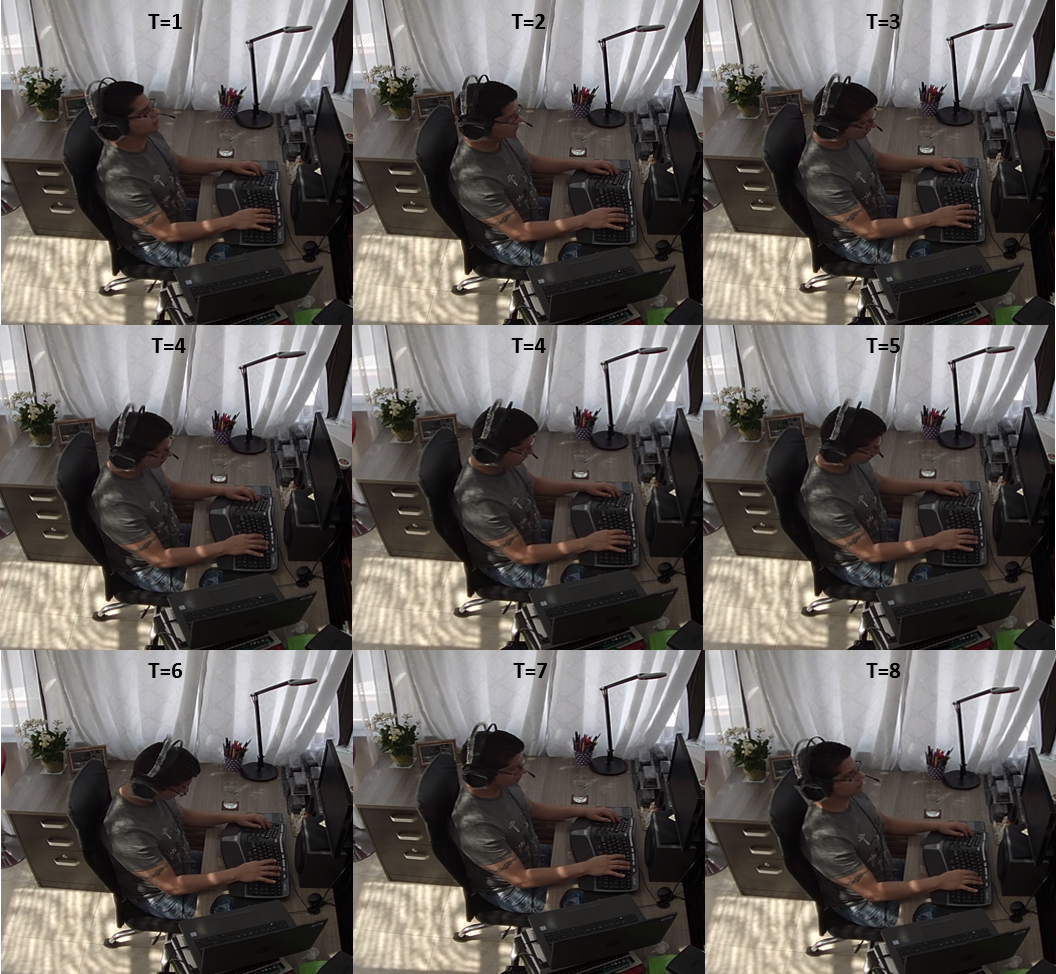
\includegraphics[width=0.8\linewidth]{./8_datasets_n_images/images/Drowsiness} 

}

\caption{Example of a drowsiness scene.}\label{fig:drowsiness}
\end{figure}

\hypertarget{activities-and-emotions-inventory}{%
\subsection{Activities and emotions
inventory}\label{activities-and-emotions-inventory}}

\textbf{This sections will introduce a table were is an inventory of
activities and emotions that can be tracked by camera}.Lorem ipsum dolor
sit amet, consectetur adipiscing elit, sed eiusmod tempor incidunt ut
labore et dolore magna aliqua. Ut enim ad minim veniam, quis nostrud
exercitation ullamco laboris nisi ut aliquid ex ea commodi consequat.
Quis aute iure reprehenderit in voluptate velit esse cillum dolore eu
fugiat nulla pariatur. Excepteur sint obcaecat cupiditat non proident,
sunt in culpa qui officia deserunt mollit anim id est laborum.

\begin{Shaded}
\begin{Highlighting}[]
\CommentTok{##}
\CommentTok{##}
\CommentTok{##Here there will be code to print}
\CommentTok{##tables from files.}
\CommentTok{##}
\CommentTok{##}
\CommentTok{##The table size will be approximately of this }
\CommentTok{##code chunk size}
\CommentTok{##}
\CommentTok{##}
\end{Highlighting}
\end{Shaded}


\end{document}
